\chapter{Inteligência artificial}\label{cap:ia} % ou aprendizado de máquina?
\section{Introdução}\label{sec:ia_intro}
Redes neurais artificiais são alguns tipos de modelos computacionais do cérebro. Tratam-se da interconexão entre unidades de processamento, geralmente neurônios artificiais. Os tipos de rede variam com o tipo de aprendizado e a arquitetura. Alguns tipos de aprendizado são os seguintes:

\begin{description}
	\item[Aprendizado supervisionado] Mapeia as entradas e saídas baseado em pares de entrada-saída de exemplo, que são rotulados (uma entrada tem a sua saída definida)
	\item[Aprendizado não-supervisionado] Aprende padrões de dados não rotulados
\end{description}

Existem diversos tipos de redes neurais artificiais, e algumas delas estão mostradas na Figura~\ref{fig:neuraltypes}.

\begin{figure}[htb!]
	\centering
	\caption{Alguns tipos de redes neurais}
	\label{fig:neuraltypes}
	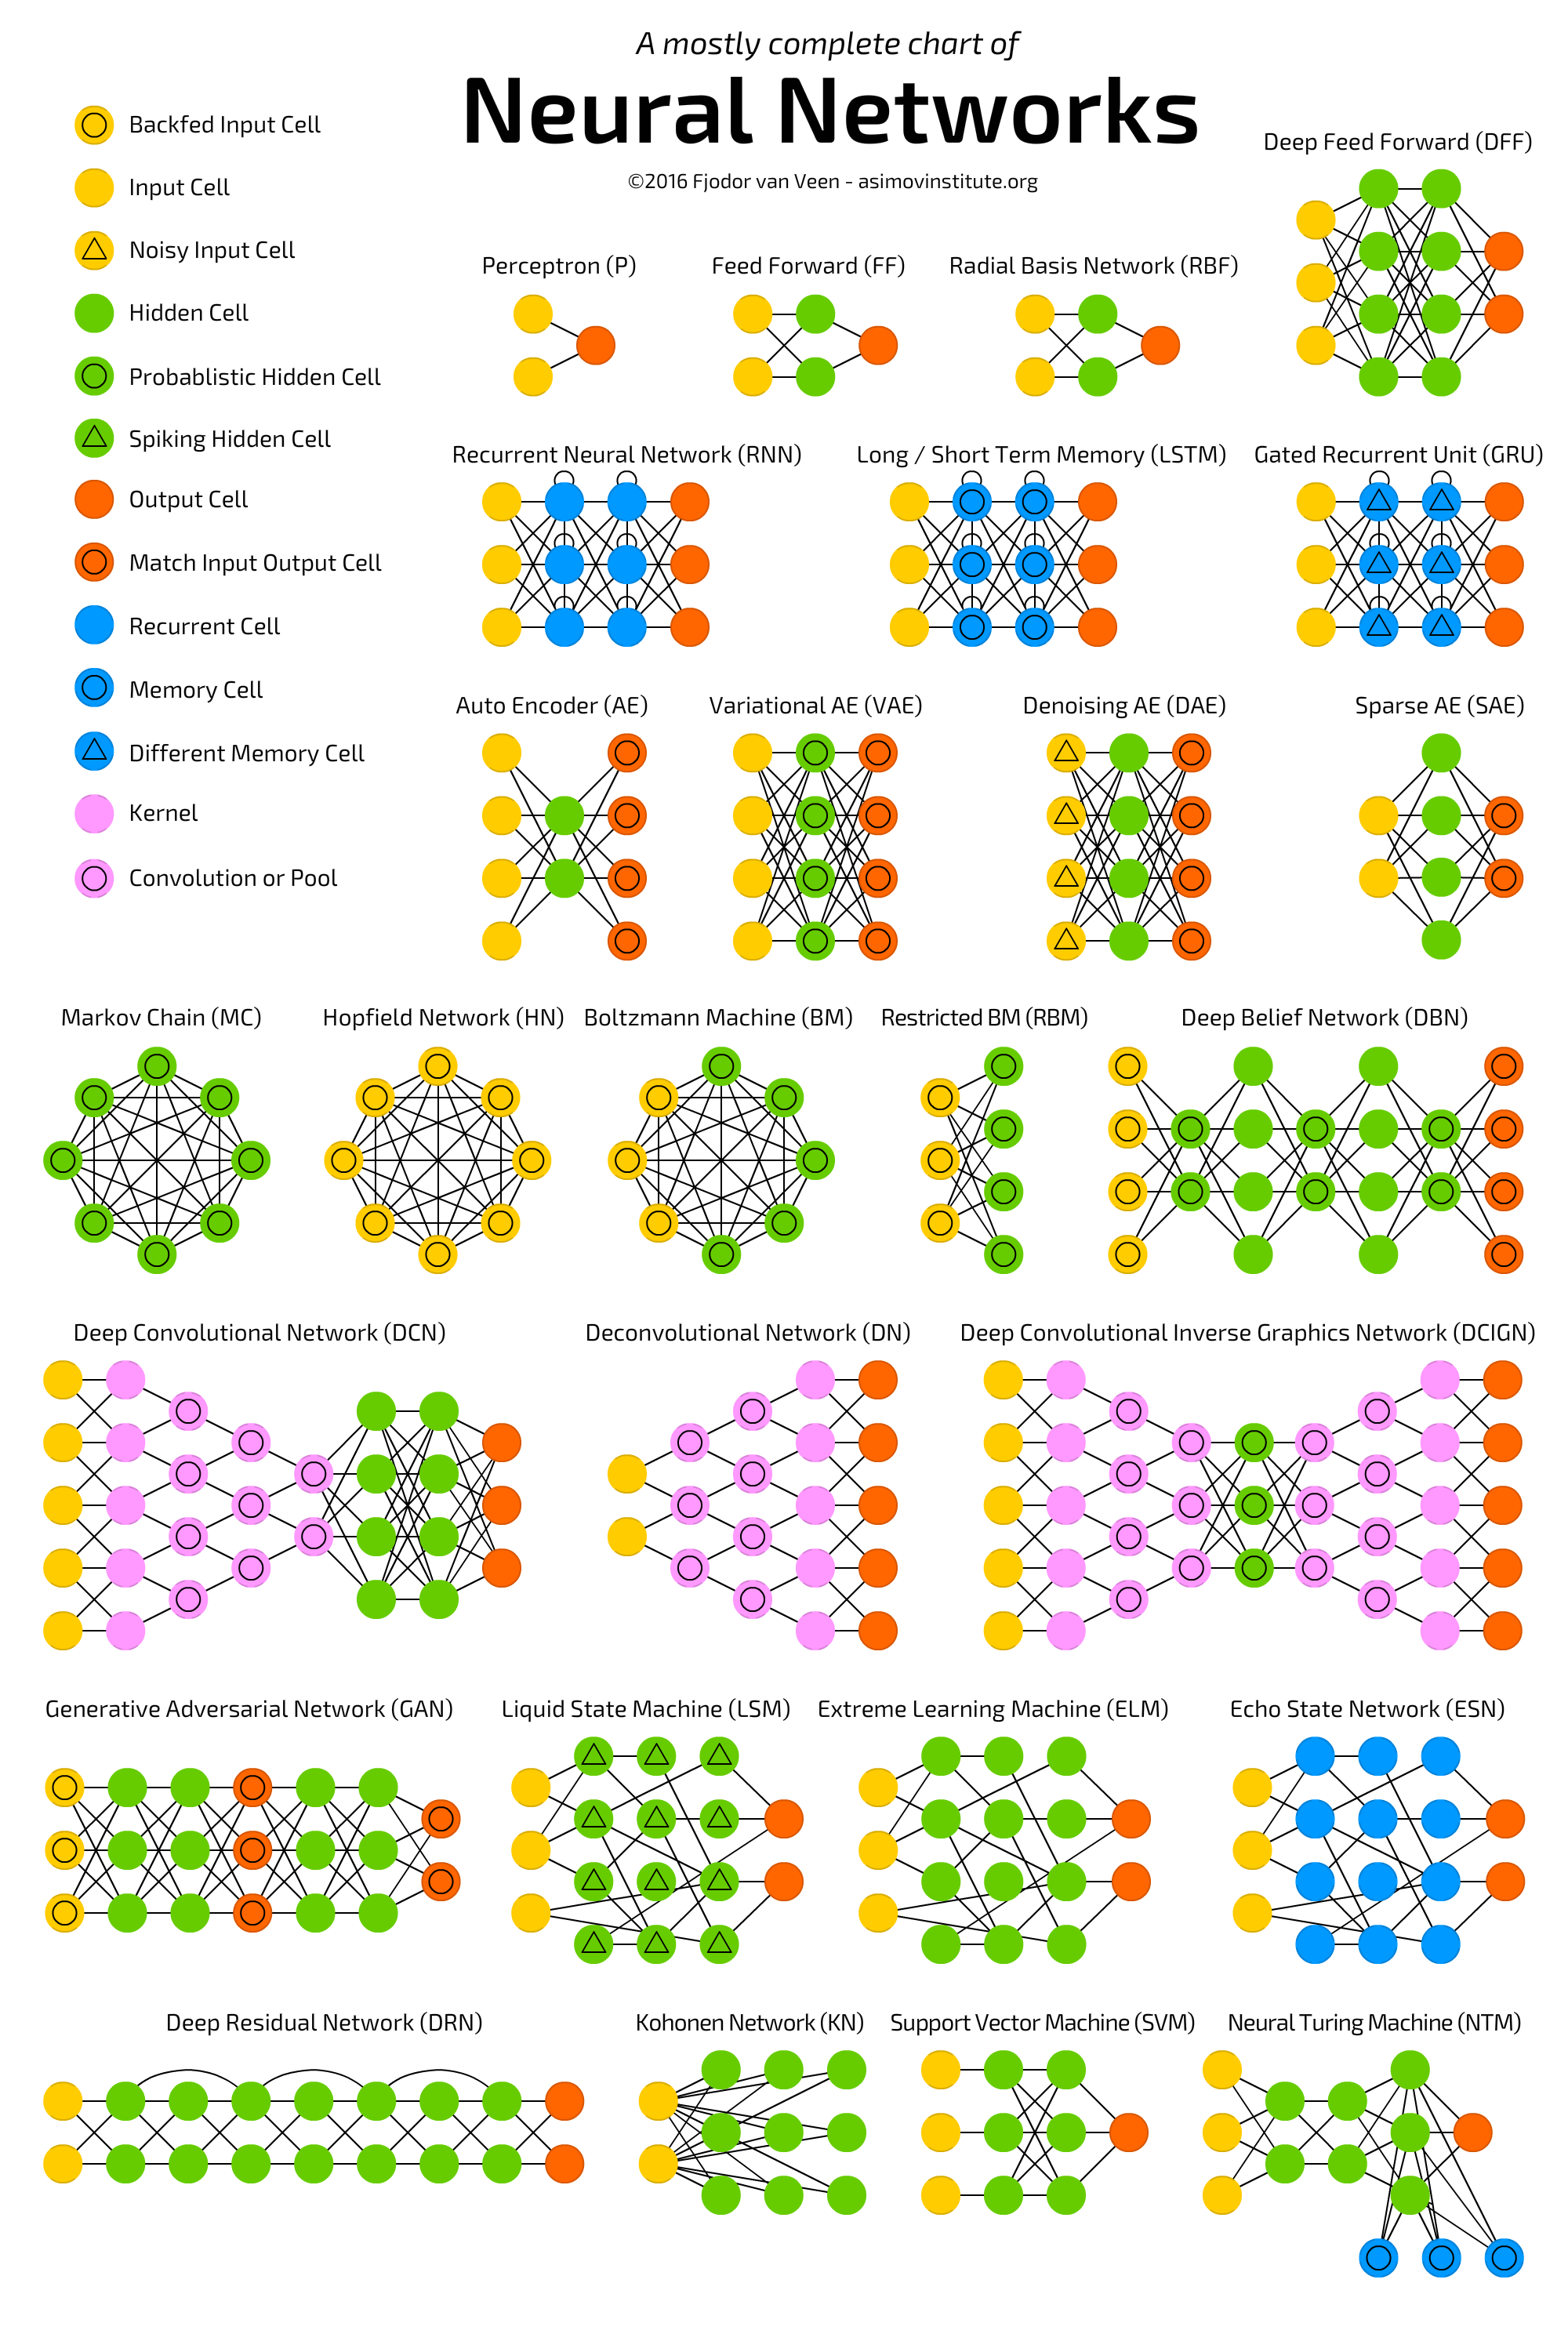
\includegraphics[width=0.34\linewidth]{figs/neural_types}
\end{figure}

Alguns desses tipos são descritos abaixo:

\begin{description}
	\item[Perceptron] Primeiro modelo de neurônio artificial. É um classificador binário com uma função de ativação do tipo degrau
	\item[Perceptron de múltiplas camadas (MLP, \textit{Multilayer perceptron})] Combinação de vários neurônios do tipo perceptron em pelo menos três camadas: uma de entrada, uma oculta e uma de saída (Figura~\ref*{fig:modelosmlp}). Utiliza a técnica de aprendizado chamada \textit{backpropagation}, onde as atualizações dos pesos é feita da camada de saída em direção à de entrada. A grande maioria das redes neurais artificiais é derivada da MLP
	\item[Redes neurais profundas] Rede neural com uma grande quantidade de camadas ocultas. Alguns subtipos incluem as \textbf{Redes neurais recorrentes}, em que os dados fluem em qualquer direção, permitindo os neurônios enviarem \textit{feedback} uns para os outros (a rede Hopfield é uma delas), e as \textbf{Redes neurais convolucionais}, que aplicam uma operação de convolução e são bastante usadas em tarefas de visão computacional
	\item[Redes neurais de disparo (SNN, \textit{Spiking Neural Networks})] Redes onde a unidade computacional é um neurônio de disparo
\end{description}

\begin{figure}[htb!]
	\centering
	\caption[Modelos básicos de neurônios e redes neurais]{Modelos básicos de neurônios e redes neurais. Em (a), o perceptron com uma função de ativação do tipo degrau; em (b), o perceptron com uma função de ativação sigmoide; em (c), uma rede neural com uma camada oculta}
	\label{fig:modelosmlp}
	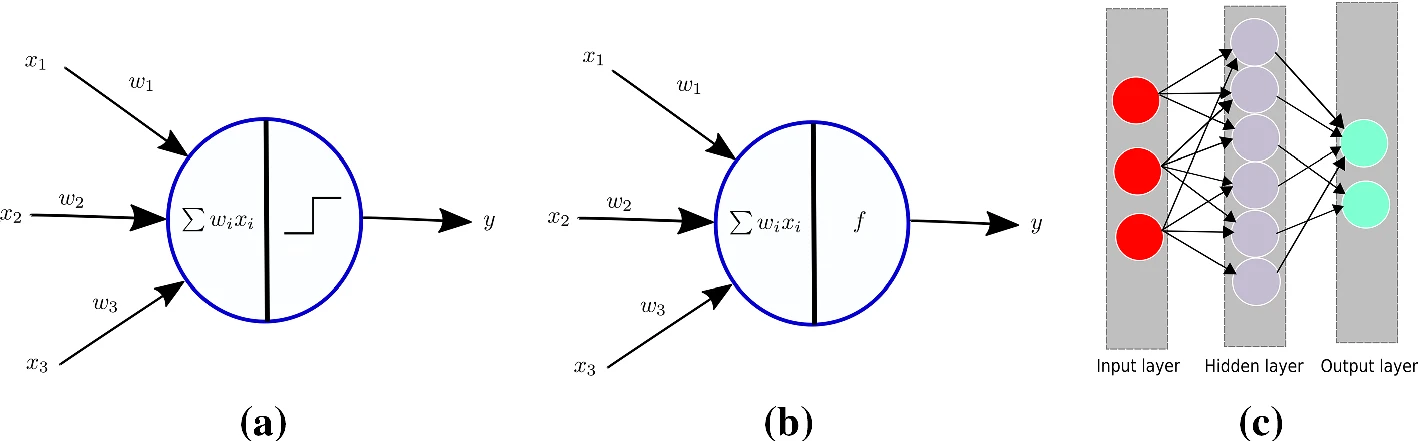
\includegraphics[width=0.9\linewidth]{figs/modelos_mlp}
\end{figure}


\section{Redes neurais}\label{sec:redesneurais}
\subsection{Redes \textit{feed-foward}}
% backprop/grad desc

\subsection{Redes recorrentes}
% lstm

\section{Redes neuromórficas}\label{sec:redesneuromorficas}
% estado da arte
% hardware neuromórfico (von-neumann vs neuromorfico)

\begin{itemize}
	\item Redes neurais de disparo usam neurônios de disparo como unidades de computação, como os modelos \textit{Leaky integrate-and-fire} (LIF) e o modelo de Izhikevich
	\item As unidades de computação são conectadas entre si e interagem através das sinapses (Figura~\ref{fig:sinapse})
\end{itemize}

\begin{figure}[htb!]
	\centering
	\caption[Neurônios pré e pós sinápticos conectados através de uma sinapse]{Neurônios pré (verde) e pós (roxo) sinápticos conectados através de uma sinapse. Os neurotransmissores (círculos vermelhos) são liberados do axônio pré-sinaptico para o dendrito pós-saptico, gerando potenciais pós-sinapticos que podem ser excitatórios (EPSP) ou inibitórios (IPSP). No neurônios pós-sinaptico os potenciais de todos os dendritos são somados e, dependendo do valor total, um potencial de ação (AP) pode ser gerado}
	\label{fig:sinapse}
	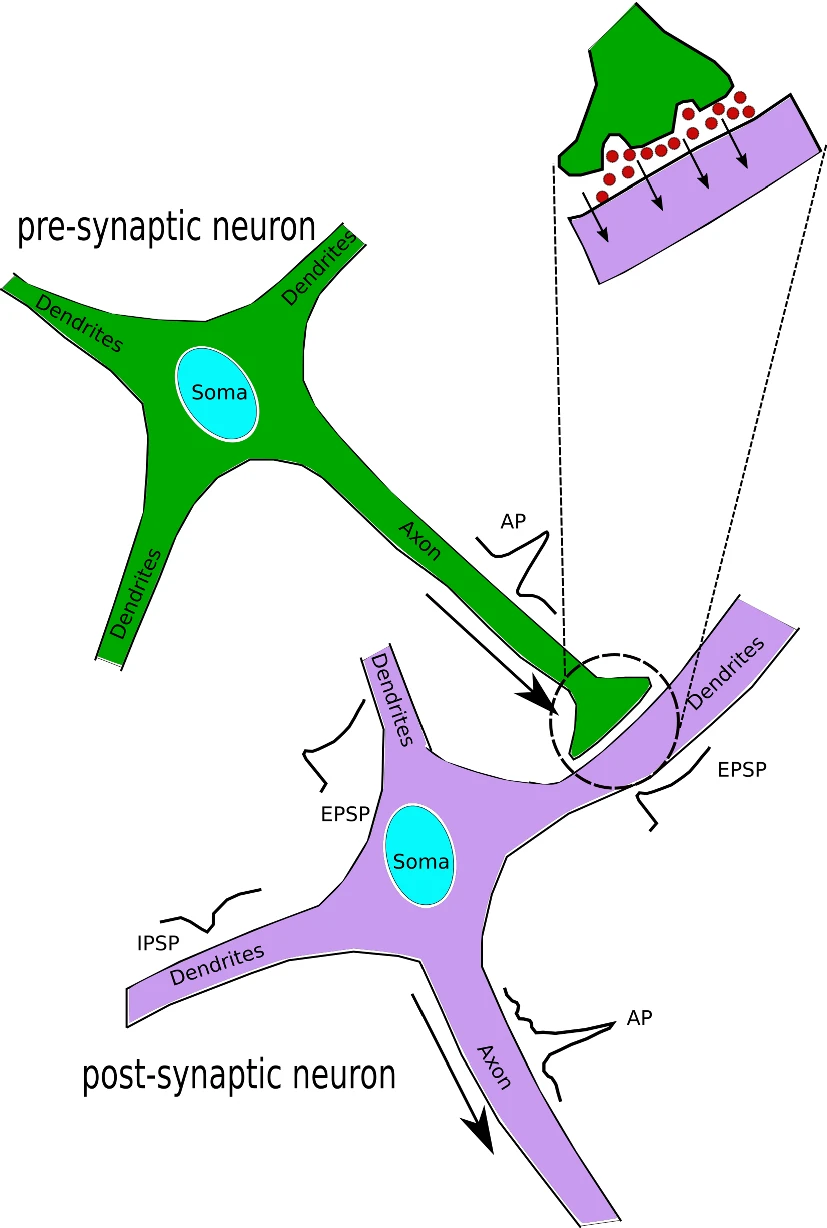
\includegraphics[width=0.3\linewidth]{figs/sinapse}
\end{figure}

\subsection{Processamento de informação}
\begin{itemize}
	\item A informação recebida pelas redes precisa ser codificada, e dois métodos para isso são:
	\begin{description}
		\item[Codificação de taxa] A taxa de disparo dos neurônios é usada. A taxa pode ser calculada como a média temporal (quantidade de disparos por intervalo de tempo), média de disparos em \textit{trials} diferentes, dentre outras maneiras
		\item[Codificação de tempo de disparo] O instante exato de ocorrência de disparos individuais é usado. Dentre os tipos de codificação nesse caso incluem-se o tempo do primeiro disparo (o tempo entre o início do estímulo e a ocorrência do primeiro disparo), a codificação de ordem (a ordem em que os neurônios disparam é o código), a codificação de latência (a diferença de tempo entre os disparos), dentre outras
	\end{description}
	\item Os critérios para seleção do método de codificação variam por diferentes aspectos, como a \textbf{minimização da perda de informação após a decodificação} e o \textbf{aumento da acurácia de previsão/classificação}
\end{itemize}

\subsection{Aprendizado das redes de disparo}
\begin{itemize}
	\item Para cada tipo de codificação citada acima, um método de aprendizado é empregado, que são:
	\begin{description}
		\item[Aprendizado baseado em taxa] Uma variação do método \textit{backpropagation} é usada aqui, relacionando as ativações das unidades das redes neurais com as taxas de disparo
		\item[Aprendizado baseado em disparo] Utiliza a plasticidade dependente de tempo de disparo (STDP, \textit{spike-timing dependent plasticity}),onde os pesos das conexões sinapticas são proporcionais ao grau de relação entre os tempos de disparo pré e pós-sinapticos (Figura~\ref{fig:stdp})
	\end{description}
\end{itemize}

\begin{figure}[htb!]
	\centering
	\caption{Conceito da STDP}
	\label{fig:stdp}
	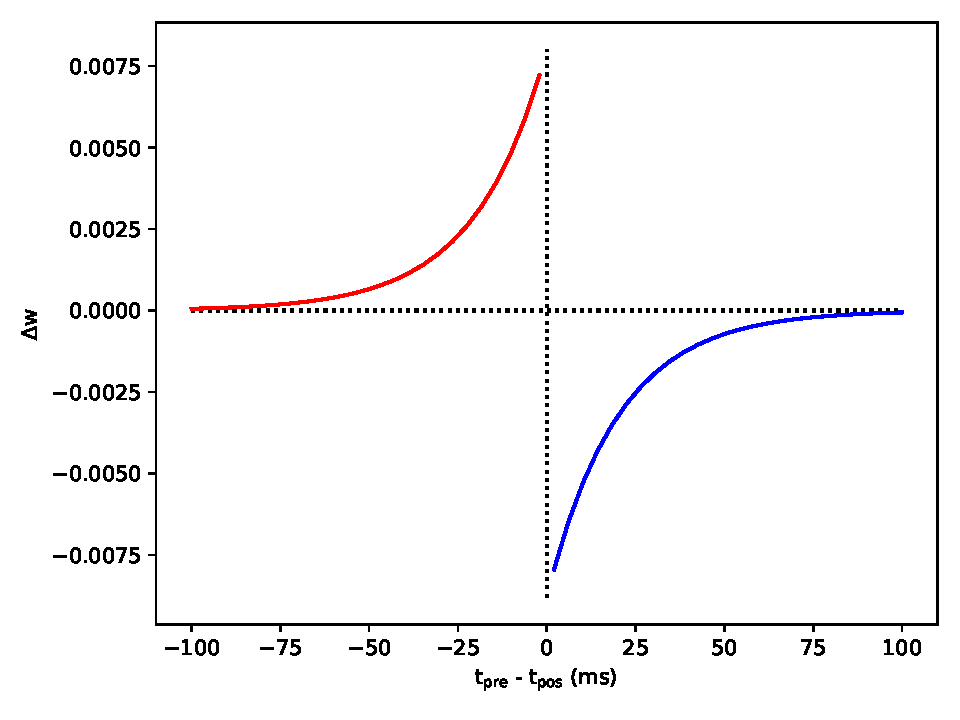
\includegraphics[width=0.7\linewidth]{figs/stdp}
\end{figure}



% pensar onde colocar os simuladores
% \section{Simuladores neuronais}\label{sec:simuladores}
